\onecolumn
\section{Power analysis}
\label{sec:power}

In this section, we'll calculate the variance of our different annotation schemes.

\newcommand{\xh}{\hat{x}}
\newcommand{\xb}{\bar{x}}
\newcommand{\yh}{\hat{y}}
\newcommand{\yb}{\bar{y}}
\newcommand{\rh}{\hat{r}}
\newcommand{\ph}{\hat{p}}

Let $\sC$ be a corpus (our ``population'') that we wish to compute statistics over
and $\sP$ be the population of pooled contexts, 
  with $r \eqdef \Pr(c \in \sP \given c \in \sC)$ (the recall of the pool).

Let $E$ be a randomly drawn subset of $\sC$ with $n_E$ samples for exhaustive annotation and
    $P$ be a randomly drawn subset of $\sP$ with $n_P$ samples for pooling annotation.

\begin{figure}
  \begin{subfigure}{0.49\textwidth}
    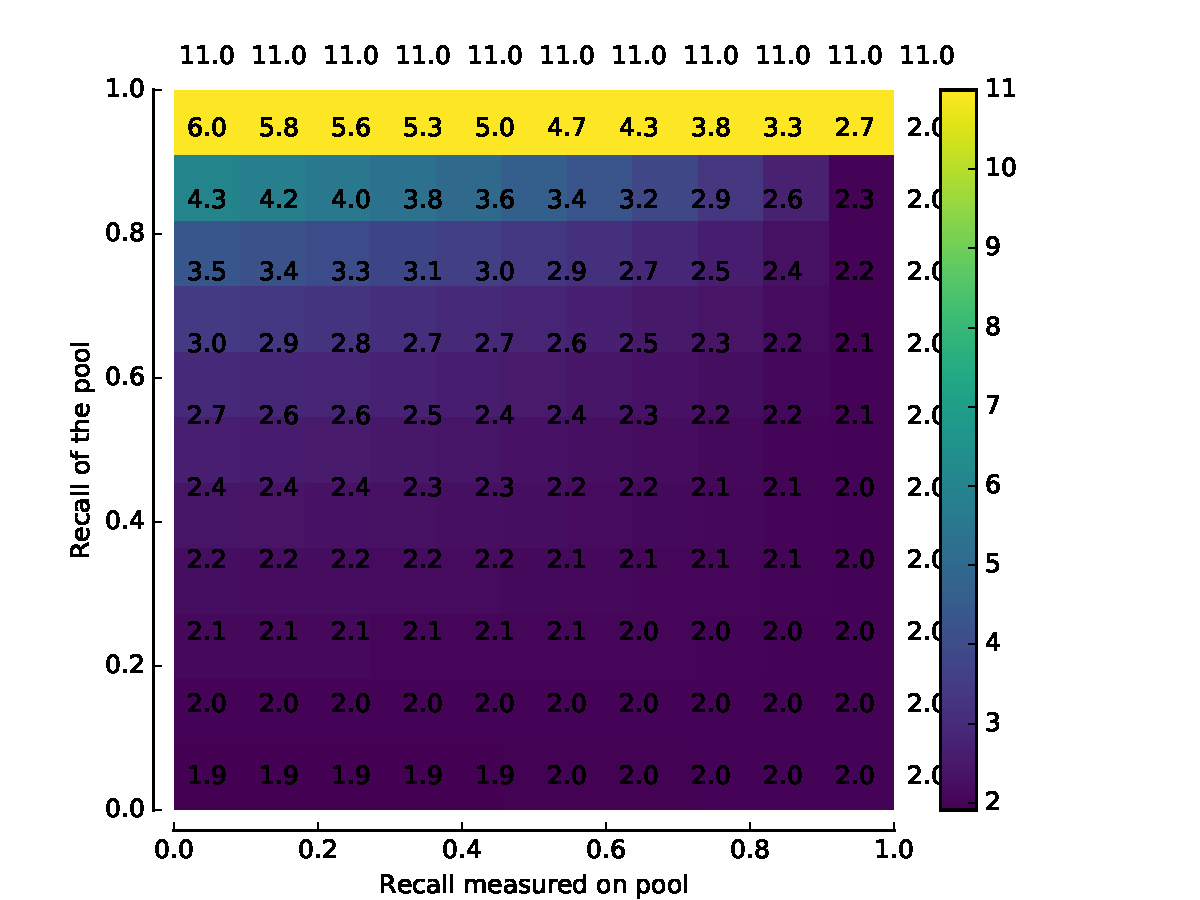
\includegraphics[width=\textwidth]{figures/variance-ratio-pool}
    \caption{\label{fig:pool-for-corpus} The relative efficiency of using pooled annotations versus exhaustive annotation, assuming that there are twice as many pooled annotations as there are exhaustive annotations.}
  \end{subfigure}
  \hfill
  \begin{subfigure}{0.49\textwidth}
    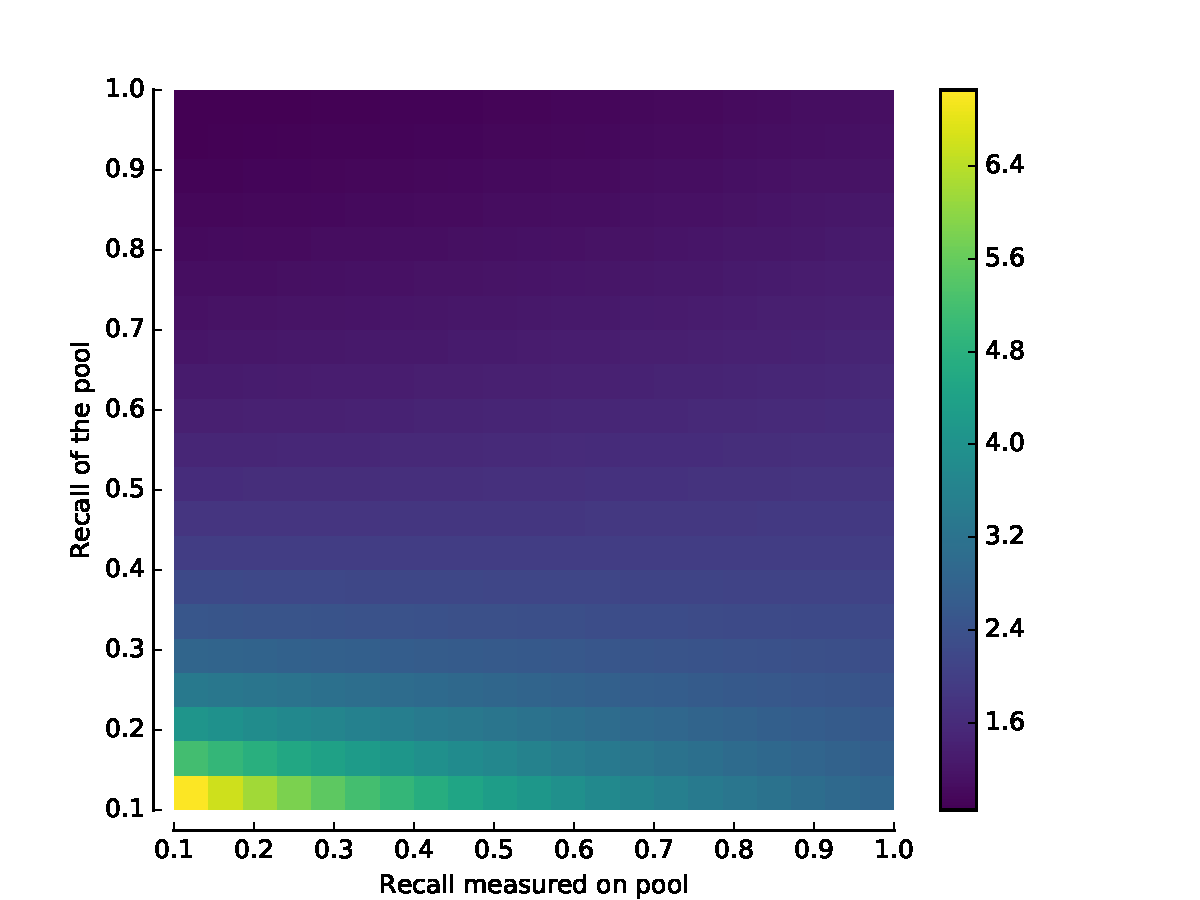
\includegraphics[width=\textwidth]{figures/variance-ratio-unassessed}
    \caption{\label{fig:pool-for-unassessed} The relative efficiency of using unassessed annotations versus exhaustive annotation, assuming that there are twice as many pooled annotations and ten times as many unassessed contexts as there are exhaustive annotations.}
  \end{subfigure}
\end{figure}

\begin{lemma}[Relative efficiency of using pooled annotations to compute corpus statistics] 
  % Define all the variables
  Let $x$ be a statistic that we wish to compute on $\sC$ (e.g.\ recall),
    $\rh$ be an unbiased estimator of $r$ on $E$ with variance $\sigma_r^2$,
    $\yh_p$ be an unbiased estimator of $x$ on $P$ with variance $\sigma_y^2$,
  then $\xh_p = \rh \yh_p$ is an unbiased estimator of $x$ on $P$ with variance
  $$
  \sigma_p^2 = \sigma_r^2 \sigma_y^2 + y^2 \sigma_r^2 + r^2 \sigma_r^2.
  $$

  Furthermore, if $\xh_e$ be an unbiased estimator of $x$ on $E$ with variance $\sigma_e^2$,
  the relative efficiency of $\xh_p$ with respect to $\xh_e$ is,
  \begin{align*}
  \frac{\sigma_e^2}{\sigma_p^2}
  &\approx \frac{1-x}
      {
      y (1-r) + \frac{n_E}{n_P} r (1-y)
      }.
  \end{align*}
  \figureref{pool-for-corpus} shows 
\end{lemma}
\begin{proof}
  \begin{align*}
    \sigma_e^2 &= \frac{x (1-x)}{n_E + 1} \\
    \sigma_r^2 &= \frac{r (1-r)}{n_E + 1} \\
    \sigma_y^2 &= \frac{y (1-y)}{n_P + 1} \\
    \sigma_p^2 
    &\approx y^2 \frac{r (1-r)}{n_E + 1} + r^2 \frac{y (1-y)}{n_P + 1} \\
    &= x^2 \left( \frac{(1-r)/r}{n_E + 1} + \frac{(1-y)}{n_P + 1} \right).
  \end{align*}
\end{proof}

\begin{lemma}[Relative efficiency of using unassessed pooled output to compute corpus statistics]
  \todo{What about dependencies of $P_i$?}
  % Define all the variables
  Let $x$ be a statistic that we wish to compute on $\sC$ (e.g.\ recall) that is $0$ outside of $\sP$,
    $\rh$ be an unbiased estimator of $r$ on $E$ with variance $\sigma_r^2$,
    $\sP_1, \dots \sP_m$ be partitions of the pool $\sP$ such that $p_i \eqdef \Pr(c \in \sC \given c \in  \sP_i)$ with $P_1, \dots, P_m$ be corresponding partitions of the sample $P$ with sizes $n_1, \dots, n_m$,
    $\ph_i, \dots, \ph_m$ be estimates of $p_i$ on $E$ with variances $\pi^2_i$,
    and $y_1, \dots y_n$ be estimates of the statistic $x$ on $\sP_i$ with variances $\sigma_i^2$.
    Then, $$\xh_u = \rh \frac{\sum_{i=1}^n \ph_i^2 |P_i| \yh_i}{\sum_{i=1}^n \ph_i |P_i|},$$ is unbiased estimator of $x$ with variance,
  $$
  \sigma_u^2 = \sigma_r^2 \sigma_y^2 + y \sigma_r^2 + r \sigma_r^2.
  $$

  Furthermore, if $\xh_e$ be an unbiased estimator of $x$ on $E$ with variance $\sigma_e^2$,
  the relative efficiency of $\xh_p$ with respect to $\xh_e$ is,
  \begin{align*}
    \frac{\sigma_e^2}{\sigma_u^2}
    &\approx \frac{1-x
      }{
        \frac{9 r(1-p)y}{n_P/n_E}  +
        \frac{4 rp(1-y)}{n_U/n_E} +
          (1-r)py
        }.
  \end{align*}
\end{lemma}
\begin{proof}
  We would like to estimate $\E_{\sC}[x]$, which can be expressed as follows,
  \begin{align*}
    \E_{\sC}[x] 
    &= \Pr(c \in \sP \intersection \sC \given c \in \sC) ~ \E_{\sP \intersection \sC}[x] 
    + \Pr(c \in \neg\sP \intersection \sC \given c \in \sC) ~ \E_{\neg\sP \intersection \sC }[x] \\
    &= r \E_{\sP}[x] + 0.
  \end{align*}
  $\sP$ can be further partitioned into $(\sP_i)$,
  \begin{align*}
    \E_{\sC}[x] 
    &= r \sum_{i=1}^n \Pr(c \in \sP_i \intersection C \given c \in \sP \intersection C) \E_{\sP_i \intersection \sC}[x].
  \end{align*}

  We don't know how to sample from $\sP_i \intersection \sC$, but we can use importance reweighting to transform estimates from $\sP_i$:
  \begin{align*}
    \E_{\sP_i \intersection \sC}[x] 
      &= \E_{\sP_i} \left[ \frac{\Pr(x \in \sC)}{x \in \sP_i} x \right] \\
      &= \E_{\sP_i}[p_i x] \\
      &= p_i y_i.
  \end{align*}
  Furthermore, $\Pr(c \in \sP_i \intersection C \given c \in \sP \intersection C) = \frac{p_i |\sP_i|}{\sum_{j=1}^n p_j |\sP_j|}$, giving us the final result,
  \begin{align*}
    \E_{\sC}[x] 
    &= r \frac{\sum_{i=1}^n p_i^2 |P_i| y_i}{\sum_{i=1}^n p_i |P_i|}.
  \end{align*}

  It is easy to see that $\E[\xh_u]$ is equal to the quantity above and hence is an unbiased estimator of $x$.

  Now, let's evaluate what the variance of $\xh_u$ is.
  Let $z \eqdef \frac{\sum_{i=1}^n \ph_i^2 |P_i| \yh_i}{\sum_{i=1}^n \ph_i |P_i|}$, the pooled estimate of recall.
  Using \reflem{variance-ratio-average}, where our two sequences are $|P_i| \ph_i$ and $\frac{\yh_i}{|P_i|}$, with means $|P_i| p_i$ and $\frac{y_i}{|P_i|}$ and variances $|P_i|^2 \pi_i^2$ and $\frac{\sigma_i^2}{|P_i|^2}$,
  \begin{align*}
    \sigma_z &\approx 
        \frac{p^2 y^2}{m} 
        {\left(1 + \frac{\pi^2}{p^2} \right)}^2
        \left(
          9 \frac{\pi^2}{p^2} +
          4 \frac{\sigma^2}{y^2}
          \right),
  \end{align*}
  where we have taken $p = \max_{i}(p_i)$, $y = \max_{i}(y_i)$, $\pi = \max_{i}(\pi_i)$, $\sigma = \max_{i}(\sigma_i)$.

  Using a Bernoulli assumption on $p$ and $y$, i.e., 
  \begin{align*}
    \pi^2 &= \frac{p (1-p)}{n_P/m} \\
    \sigma^2 &= \frac{y (1-y)}{n_U/m},
  \end{align*}
  we get
  \begin{align*}
    \sigma_z &\approx 
        p^2 y^2
        {\left(1 + \frac{{(1-p)}^2}{n_P} \right)}^2
        \left(
        \frac{9 (1-p)/p}{n_P}  +
        \frac{4 (1-y)/y}{n_U}
          \right) \\
        &\approx
        p^2 y^2
        \left(
        \frac{9 (1-p)/p}{n_P}  +
        \frac{4 (1-y)/y}{n_U}
          \right).
  \end{align*}

  Finally, the variance of $u$ is 
  \begin{align*}
  \sigma_u^2 &= r^2 \sigma_z^2 + z^2 \sigma_r^2 \\
        &\approx r^2 p^2 y^2
        \left(
        \frac{9 (1-p)/p}{n_P}  +
        \frac{4 (1-y)/y}{n_U}
          \right) +
          p^2 y^2 r^2 \frac{(1-r)/r}{n_E} \\
        &= x
        \left(
        \frac{9 r(1-p)y}{n_P}  +
        \frac{4 rp(1-y)}{n_U}
          \frac{(1-r)py}{n_E}
          \right).
  \end{align*}

  Using the same Bernoulli assumption on $\xh_e$, we get that $\sigma^2_e = \frac{x (1-x)}{n_E}$.
  The relative efficiency of $\xh_u$ versus $\xh_e$ is approximately,
  \begin{align*}
    \frac{\sigma_e^2}{\sigma_u^2}
    &\approx \frac{1-x
      }{
        \frac{9 r(1-p)y}{n_P/n_E}  +
        \frac{4 rp(1-y)}{n_U/n_E} +
          (1-r)py
        }.
  \end{align*}
\end{proof}

\begin{lemma}[Relative efficiency of using unassessed pooled output to compute submission statistics]
  \todo{Compute! What are dependences of $S_i$?}
  % Define all the variables
  Let $x$ be a statistic that we wish to compute on $\sS$ (e.g.\ precision) that is $0$ outside of $\sS$,
    $\sP_1, \dots \sP_m$ be partitions of the pool $\sP$ such that $p_i \eqdef \Pr(c \in \sC \given c \in  \sP_i)$ with $S_1, \dots, S_m$ be corresponding partitions of the sample $S$ with sizes $n_1, \dots, n_m$,
    $\ph_i, \dots, \ph_m$ be estimates of $p_i$ on $E$ with variances $\pi^2_i$,
    and $y_1, \dots y_n$ be estimates of the statistic $x$ on $\sP_i$ with variances $\sigma_i^2$.
    Then, $$\xh_u = \sum_{i=1}^n \ph_i \frac{|S_i|^2}{|S|^2},$$ is unbiased estimator of $x$ with variance,
  $$
  \sigma_u^2 
        = \sum_{i=1}^n \frac{|S_i|^4}{|S|^4} \pi_i^2 \\
        \le \pi^2.
  $$

  Furthermore, if $\xh_s$ be an unbiased estimator of $x$ on $S$ with variance $\sigma_s^2$,
  the relative efficiency of $\xh_u$ with respect to $\xh_s$ is,
  \begin{align*}
    \frac{\sigma_u^2}{\sigma_s^2}
    &\approx \frac{1-x
      }{
        \frac{9 r(1-p)y}{n_P/n_E}  +
        \frac{4 rp(1-y)}{n_U/n_E}
          \frac{(1-r)py}{n_E}
        }.
  \end{align*}
\end{lemma}
\begin{proof}
  We would like to estimate $\E_{\sC}[x]$, which can be expressed as follows,
  \begin{align*}
    \E_{\sC}[x] 
    &= \Pr(c \in \sP \intersection \sC \given c \in \sC) ~ \E_{\sP \intersection \sC}[x] 
    + \Pr(c \in \neg\sP \intersection \sC \given c \in \sC) ~ \E_{\neg\sP \intersection \sC }[x] \\
    &= r \E_{\sP}[x] + 0.
  \end{align*}
  $\sP$ can be further partitioned into $(\sP_i)$,
  \begin{align*}
    \E_{\sC}[x] 
    &= r \sum_{i=1}^n \Pr(c \in \sP_i \intersection C \given c \in \sP \intersection C) \E_{\sP_i \intersection \sC}[x].
  \end{align*}

  We don't know how to sample from $\sP_i \intersection \sC$, but we can use importance reweighting to transform estimates from $\sP_i$:
  \begin{align*}
    \E_{\sP_i \intersection \sC}[x] 
      &= \E_{\sP_i} \left[ \frac{\Pr(x \in \sC)}{x \in \sP_i} x \right] \\
      &= \E_{\sP_i}[p_i x] \\
      &= p_i y_i.
  \end{align*}
  Furthermore, $\Pr(c \in \sP_i \intersection C \given c \in \sP \intersection C) = \frac{p_i |\sP_i|}{\sum_{j=1}^n p_j |\sP_j|}$, giving us the final result,
  \begin{align*}
    \E_{\sC}[x] 
    &= r \frac{\sum_{i=1}^n p_i^2 |P_i| y_i}{\sum_{i=1}^n p_i |P_i|}.
  \end{align*}

  It is easy to see that $\E[\xh_u]$ is equal to the quantity above and hence is an unbiased estimator of $x$.

  Now, let's evaluate what the variance of $\xh_u$ is.
  Let $z \eqdef \frac{\sum_{i=1}^n \ph_i^2 |P_i| \yh_i}{\sum_{i=1}^n \ph_i |P_i|}$, the pooled estimate of recall.
  Using \reflem{variance-ratio-average}, where our two sequences are $|P_i| \ph_i$ and $\frac{\yh_i}{|P_i|}$, with means $|P_i| p_i$ and $\frac{y_i}{|P_i|}$ and variances $|P_i|^2 \pi_i^2$ and $\frac{\sigma_i^2}{|P_i|^2}$,
  \begin{align*}
    \sigma_z &\approx 
        \frac{p^2 y^2}{m} 
        {\left(1 + \frac{\pi^2}{p^2} \right)}^2
        \left(
          9 \frac{\pi^2}{p^2} +
          4 \frac{\sigma^2}{y^2}
          \right),
  \end{align*}
  where we have taken $p = \max_{i}(p_i)$, $y = \max_{i}(y_i)$, $\pi = \max_{i}(\pi_i)$, $\sigma = \max_{i}(\sigma_i)$.

  Using a Bernoulli assumption on $p$ and $y$, i.e., 
  \begin{align*}
    \pi^2 &= \frac{p (1-p)}{n_P/m} \\
    \sigma^2 &= \frac{y (1-y)}{n_U/m},
  \end{align*}
  we get
  \begin{align*}
    \sigma_z &\approx 
        p^2 y^2
        {\left(1 + \frac{{(1-p)}^2}{n_P} \right)}^2
        \left(
        \frac{9 (1-p)/p}{n_P}  +
        \frac{4 (1-y)/y}{n_U}
          \right) \\
        &\approx
        p^2 y^2
        \left(
        \frac{9 (1-p)/p}{n_P}  +
        \frac{4 (1-y)/y}{n_U}
          \right).
  \end{align*}

  Finally, the variance of $u$ is 
  \begin{align*}
  \sigma_u^2 &= r^2 \sigma_z^2 + z^2 \sigma_r^2 \\
        &\approx r^2 p^2 y^2
        \left(
        \frac{9 (1-p)/p}{n_P}  +
        \frac{4 (1-y)/y}{n_U}
          \right) +
          p^2 y^2 r^2 \frac{(1-r)/r}{n_E} \\
        &= x
        \left(
        \frac{9 r(1-p)y}{n_P}  +
        \frac{4 rp(1-y)}{n_U}
          \frac{(1-r)py}{n_E}
          \right).
  \end{align*}

  Using the same Bernoulli assumption on $\xh_e$, we get that $\sigma^2_e = \frac{x (1-x)}{n_E}$.
  The relative efficiency of $\xh_u$ versus $\xh_e$ is approximately,
  \begin{align*}
    \frac{\sigma_e^2}{\sigma_u^2}
    &\approx \frac{1-x
      }{
        \frac{9 r(1-p)y}{n_P/n_E}  +
        \frac{4 rp(1-y)}{n_U/n_E}
          \frac{(1-r)py}{n_E}
        }.
  \end{align*}
\end{proof}


\begin{lemma}[Benefit of combining estimators]
  Let $x_1, \dots, x_n$ be independent and unbiased estimators for a statistic $x$ with variances $\sigma_1^2, \dots \sigma_n^2$.
  Let $z = \sum_{i=1}^n \alpha_i x_i$ where $\sum_{i=1}^n \alpha_i = 1$ be a combined estimator for $x$ with minimal variance.
  Then, the relative efficiency, i.e ratio of variances, of $z$ and $x_1$ is,
  $\frac{\sigma_z^2}{\sigma_1^2} = \sum_{i=1}^n \frac{\sigma_i^2}{\sigma_1^2}$.

  In other words, relative efficiency of a combined estimator with respect
  to an original estimator is the sum of relative efficiencies of each component
  estimator with respect to the original estimator. 
\end{lemma}


\section{Basic probability lemmas}
\label{sec:probability}

% TODO: include KKT variables.
\begin{lemma}[Mean and variance of the sum of two random variables]
  \label{lem:combined-variance}
  Let $x$ and $y$ be two random variables with mean $0$, variances $\sigma^2_x$ and $\sigma^2_y$ and a correlation coefficient of $\rho$.
  Then, the estimator $z = \alpha x + (1-\alpha) y$, where $0 \le \alpha
  \le 1$ also has mean $0$ and has minimum variance $\sigma^2_z$ when
  \begin{align*}
  \alpha &= 
  \begin{cases}
    0 & \rho > \frac{\sigma_x}{\sigma_y} \\
    1 & \rho > \frac{\sigma_x}{\sigma_y} \\
    \frac{\sigma_y (\sigma_y - \rho \sigma_x)}{\sigma_x^2 + \sigma_y^2 - 2\rho \sigma_x \sigma_y} & \text{otherwise},
  \end{cases}
  &
  \sigma^2_z &= 
  \begin{cases}
    \sigma^2_y & \rho > \frac{\sigma_x}{\sigma_y} \\
    \sigma^2_x & \rho > \frac{\sigma_x}{\sigma_y} \\
    \frac{\sigma_x^2 \sigma_y^2 (1 - \rho^2)}{\sigma_x^2 + \sigma_y^2 - 2 \rho \sigma_x \sigma_y} & \text{otherwise}.
  \end{cases}
  \end{align*}

  In general, if $x_i$ are uncorrelated random variables, $z = \sum_{i} \alpha_i x_i$ where $\sum_i \alpha_i = 1$ has mean and optimal variance,
  $$\frac{1}{\sigma_z^2} = \sum_i \frac{1}{\sigma_i^2}.$$
\end{lemma}
\begin{proof}
  \newcommand{\alphab}{\bar{\alpha}}
  For notational convenience, let $\alphab \eqdef 1 - \alpha$.
  That $z$ has mean $0$ follows directly from the linearity of expectations.
  The variance of $z$ can be calculated as follows:
  \begin{align*}
    \sigma^2_z &\eqdef \var(z) 
            &= \E[z^2] - \E[z]^2 \\
            &= \E[(\alpha x+ \alphab y)^2] - 0 \\
            &= \E[\alpha^2 x^2 + \alphab^2 y^2 + 2 \alpha \alphab x y] \\
            &= \alpha^2 \sigma_x^2 + \alphab^2 \sigma_y^2 + 2 \alpha \alphab \E[x y] \\
            &= \alpha^2 \sigma_x^2 + \alphab^2 \sigma_y^2 + 2 \alpha \alphab \rho \sigma_x \sigma_y,
  \end{align*}
  using the fact that $\rho \eqdef \frac{\E[xy]}{\sigma_x \sigma_y}$.

  We introduce Lagrange multipliers $\lambda_1, \lambda_2 \ge 0$ to handle the constraint that $0 \le \alpha \le 1$,
  \begin{align*}
    \sL &= 
    \alpha^2 \sigma_x^2 + \alphab^2 \sigma_y^2 + 2 \alpha \alphab \rho \sigma_x \sigma_y
    + \lambda_1 \alpha + \lambda_2 \alphab \\
    \frac{d}{d\alpha} \sL &= 
    2 \alpha \sigma_x^2 - 2(1 - \alpha) \sigma_y^2 + 2 (1 - 2\alpha) \rho \sigma_x \sigma_y + \lambda_1 - \lambda_2
&= 
    2 (\alpha (\sigma_x^2 + \sigma_y^2 - 2 \rho \sigma_x\sigma_y) - \sigma_y^2 + \rho \sigma_x \sigma_y + \lambda'_1 - \lambda'_2),
  \end{align*}
  where $\lambda'_1$ and $\lambda'_2$ are suitably redefined to absorb the constant.

  This quantity is minimized when the gradient with respect $\alpha$ is $0$,
  \begin{align*}
    \alpha (\sigma_x^2 + \sigma_y^2 - 2\rho \sigma_x \sigma_y) &= \sigma_y^2 - \rho \sigma_x \sigma_y + \lambda'_2 - \lambda'_1 \\
    \alpha &= \frac{\sigma_y^2 - \rho \sigma_x \sigma_y + \lambda'_2 - \lambda'_1}{\sigma_x^2 + \sigma_y^2 - 2\rho \sigma_x \sigma_y} \\
    \alphab &= \frac{\sigma_x^2 - \rho \sigma_x \sigma_y - \lambda'_2 + \lambda'_1}{\sigma_x^2 + \sigma_y^2 - 2\rho \sigma_x \sigma_y}.
  \end{align*}

  The KKT conditions give us that $\lambda'_1 \alpha = 0$ and $\lambda'_2 (1-\alpha) = 0$, which implies that only one of $\lambda'_1$ or $\lambda'_2$ are non-zero.
  We can see that $\alpha = 0$ when $\sigma_y^2 - \rho \sigma_x \sigma_y < 0$, or when $\rho \ge \frac{\sigma_y}{\sigma_x}$.
  Likewise, $\alpha = 1$ when $\sigma_x^2 - \rho \sigma_x \sigma_y < 0$, or when $\rho \ge \frac{\sigma_x}{\sigma_y}$.
  This gives us the result on $\alpha$.

  The value of $\sigma_z^2$ when $\alpha = 0$ or $\alpha=1$ is simply $\sigma_y^2$ or $\sigma_x^2$.
  When $0 < \alpha < 1$, it is,
  \begin{align*}
    \sigma_z^2
            &= \frac{
            \sigma_x^2 \sigma_y^2 (\sigma_y - \rho \sigma_x)^2
            + \sigma_x^2 \sigma_y^2 (\sigma_x - \rho \sigma_y)^2
            + 2 \rho \sigma_x^2 \sigma_y^2 (\sigma_y - \rho \sigma_x) (\sigma_x - \rho \sigma_y)}{
            (\sigma_x^2 + \sigma_y^2 - 2\rho \sigma_x \sigma_y)^2
            }\\
            &= \sigma_x^2 \sigma_y^2 
            \frac{
             \sigma_y^2 + \rho^2 \sigma_x^2 - 2 \rho \sigma_x \sigma_y 
            + \sigma_x^2 + \rho^2 \sigma_y^2 - 2 \rho \sigma_x \sigma_y 
            + 2 \rho (\sigma_x \sigma_y - \rho \sigma_y^2 - \rho \sigma_x^2 + \rho^2 \sigma_x \sigma_y)}{
            (\sigma_x^2 + \sigma_y^2 - 2\rho \sigma_x \sigma_y)^2
            }\\
            &= \sigma_x^2 \sigma_y^2 
            \frac{
             (1 - \rho^2) (\sigma_x^2 + \sigma_y^2 - 2 \rho \sigma_x \sigma_y)}{
            (\sigma_x^2 + \sigma_y^2 - 2\rho \sigma_x \sigma_y)^2
            }\\
            &= 
            \frac{(1 - \rho^2) \sigma_x^2 \sigma_y^2}{
              \sigma_x^2 + \sigma_y^2 - 2\rho \sigma_x \sigma_y
            }\\
  \end{align*}
\end{proof}

\begin{lemma}[Mean and variance of the product of two random variables]
  \label{lem:variance-product}
  Let $x$ and $y$ be two independent random variables with means $\mu_x$ and $\mu_y$, and variances $\sigma^2_x$ and $\sigma^2_y$.
  Then, the estimator $z = x y$ has mean $\mu_x \mu_y$ and variance
  $$\sigma^2_z = \sigma_x^2 \sigma_y^2 + \mu_x^2 \sigma_y^2 + \sigma_x^2 \mu_y^2.$$
\end{lemma}
\begin{proof}
  If $x$ and $y$ are independent, $\E[xy] = \E[x]\E[y]$. Thus $\E[z] = \mu_x \mu_y$.

  The variance of $z$ can be calculated as follows:
  \begin{align*}
    \var(z) &= \E[z^2] - {\E[z]}^2 \\
    &= \E[{(xy)}^2] - {\E[xy]}^2 \\
            &= \E[x^2] \E[y^2] - {\E[x]}^2 {\E[y]}^2 \\
            &= (\sigma^2_x + \mu_x^2)(\sigma^2_y + \mu_y^2) - \mu_x^2 \mu_y^2 \\
            &= \sigma_x^2 \sigma_y^2 + \mu_x^2 \sigma_y^2 + \sigma_x^2 \mu_y^2 + \mu_x^2 \mu_y^2 - \mu_x^2 \mu_y^2 \\
            &= \sigma_x^2 \sigma_y^2 + \mu_x^2 \sigma_y^2 + \sigma_x^2 \mu_y^2.
  \end{align*}
\end{proof}

\begin{lemma}[Mean and variance of the ratio of two random variables]
\label{lem:variance-ratio}
  Let $x$ and $y$ be two random variables with means $\mu_x$ and $\mu_y$, variances $\sigma^2_x$ and $\sigma^2_y$ and correlation $\rho$. Furthermore, $y$ has positive support (i.e.\ $y > 0$). 
  Then, $z = x / y$ approximately has mean $\mu_x / \mu_y$ and variance
  $$\sigma^2_z \approx \frac{\mu^2_x}{\mu_y^2} \left(\frac{\sigma_x^2}{\mu_x^2} 
    + 2\rho \frac{\sigma_x \sigma_y}{\mu_x \mu_y}
    + \frac{\sigma_y^2}{\mu_y^2} \right).$$

\end{lemma}
\begin{proof}
  Let $f(x,y) = \frac{x}{y}$.
  Even if $x$ and $y$ are independent, $\E[f(x,y)]$ is not strictly $f(\E[x],\E[y])$.
  However, taking a first-order Taylor expansion around $(\mu_x, \mu_y)$, we get
  \begin{align*}
    \E[f(x,y)] 
     &\approx f(\mu_x,\mu_y) + f_x'(\mu_x, \mu_y) \E[x - \mu_x] + f'_y(\mu_x, \mu_y) \E[y - \mu_y] \\
     &= \frac{\mu_x}{\mu_y}.
  \end{align*}

  Taking a similar approach to calculate variance, we get,
  \begin{align*}
    \var(f(x,y)) 
             &\approx \E[(f(x,y) - \E[f(x,y)])^2] \\
             &= \E[{(f(\mu_x,\mu_y) + f'_x(\mu_x, \mu_y) (x - \mu_x) + f'_y(\mu_x, \mu_y) (y - \mu_y) - f(\mu_x, \mu_y))}^2] \\
             &= f'_x(\mu_x, \mu_y)^2 \E[(x - \mu_x)^2] + f'_y(\mu_x, \mu_y)^2 \E[(y - \mu_y)^2] 
              + 2 f'_x(\mu_x, \mu_y)f'_y(\mu_x, \mu_y) \E[(x - \mu_x)(y - \mu_y)]\\
             &= f'_x(\mu_x, \mu_y)^2 \sigma_x^2 + f'_y(\mu_x, \mu_y)^2 \sigma_y^2
              + 2 f'_x(\mu_x, \mu_y)f'_y(\mu_x, \mu_y) \rho \sigma_x \sigma_y.
  \end{align*}
  Noting that $f'_x(\mu_x, \mu_y) = \frac{1}{\mu_y}$ and that $f'_y(\mu_x, \mu_y) = -\frac{\mu_x}{\mu_y^2}$, we get,
  \begin{align*}
    \var(f(x,y)) 
    &\approx \frac{\sigma_x^2}{\mu_y^2} + \frac{\sigma_y^2 \mu_x^2}{\mu_y^4}
    + 2 \frac{\mu_x}{\mu_y^3} \rho \sigma_x \sigma_y \\
    &= \frac{\mu^2_x}{\mu_y^2} \left(\frac{\sigma_x^2}{\mu_x^2} 
    + 2\rho \frac{\sigma_x \sigma_y}{\mu_x \mu_y}
    + \frac{\sigma_y^2}{\mu_y^2} \right).
 \end{align*}
\end{proof}

\begin{lemma}[Mean and variance of a importance-weighted estimate.]
\label{lem:variance-ratio-average}
  Let $p_i$ and $q_i$ be two sets of independent random variables with means $\mu$ and $\xi$ and variances $\sigma^2$ and $\pi^2$ respectively.
  Then, $z = \frac{\sum_{i=1}^n p^2_i q_i}{\sum_{i=1}^n p_i}$ has mean $\xi$ and variance,
  $$\sigma^2_z \approx
  \frac{\mu^2 \xi^2}{n} {\left( 1 + \frac{\sigma^2}{\mu^2} \right)}^2
             \left(
                9 \frac{\sigma^2}{\mu^2} + 4 \frac{\pi^2}{\xi^2}
                \right).$$
\end{lemma}
\begin{proof}
  From \reflem{variance-ratio} we have that
  $$\sigma^2_z \approx \frac{\mu^2_x}{\mu_y^2} \left(\frac{\sigma_x^2}{\mu_x^2} 
    + 2\rho \frac{\sigma_x \sigma_y}{\mu_x \mu_y}
    + \frac{\sigma_y^2}{\mu_y^2} \right),$$
    where $x = \frac{1}{n}\sum_{i=1}^n p_i^2 q_i$ and $y = \frac{1}{n}\sum_{i=1}^n p_i$.

  In the following, we will make Gaussian assumptions on any moments $>3$ and ignore variance squared terms, e.g. $\sigma^4 \approx 0$.
  Thus,
  \begin{align*}
    \E[x^3] &\approx 3\sigma_x^2 \mu_x + \mu_x^3 \\
    \E[x^4] &\approx 6\sigma_x^2 \mu_x^2 + \mu_x^4 \\
    \var[x^2] &= \E[x^4] - {\E[x^2]}^2 \\
              &\approx 6\sigma_x^2 \mu_x^2 + \mu_x^4 - {(\mu_x^2 + \sigma_x^2)}^2 \\
              &= 4\sigma_x^2 \mu_x^2 
  \end{align*}
  
  Let us solve for each term independently,
  \begin{align*}
    \mu_x &= (\sigma^2 + \mu^2) \xi \\
          &= \mu^2 \xi (1 + \frac{\sigma^2}{\mu^2}) \\
    \mu_y &= \mu \\
    \sigma_x^2 &\approx \frac{1}{n} (\var[{p_i^2}] \xi^2 + {(\sigma^2 + \mu^2)}^2 \pi^2) \\
               &<  \frac{1}{n} (4 \mu^2 \sigma^2 \xi^2 + 4 \mu^4 \pi^2) \\
               &= \frac{4}{n} \mu^4 \xi^2 \left( \frac{\sigma^2}{\mu^2}  + \frac{\pi^2}{\xi^2} \right) \\
    \sigma_y^2 &= \frac{1}{n} \sigma^2.
  \end{align*}

  Finally, for $\rho \sigma_x \sigma_y = \E[x y] - \mu_x \mu_y$, we get,
  \begin{align*}
      \rho \sigma_x \sigma_y &\eqdef \E[(\sum_{i=1}^n p^2_i q_i)(\sum_{j=1}^n p_j)] -  \E[(\sum_{i=1}^n p^2_i q_i)]\E[(\sum_{j=1}^n p_j)]\\
           &= \sum_{i=1}^n \E[p^3_i] \E[q_i] - \E[p^2_i] \E[q_i] \E[p_i] \\
           &= \sum_{i=1}^n (\E[p^3_i] - \E[p^2_i] \E[p_i]) \E[q_i] \\
           &= \frac{1}{n} (3\sigma^2 \mu + \mu^3 - (\sigma^2 + \mu^2) \mu) \xi \\
           &= \frac{2}{n} \sigma^2 \mu \xi.
  \end{align*}
  noting that all other terms are 0.

  Putting all of these together, we get,
  \begin{align*}
    \sigma_z^2 &< 
           \mu^2 \xi^2 (1 + \frac{\sigma^2}{\mu^2})^2
           \left(
           \frac{4}{n} (\frac{\sigma^2}{\mu^2} + \frac{\pi^2}{\xi^2})
              +
              \frac{4}{n} \frac{\sigma^2 \mu \xi}{\mu^2 \xi \mu}
              +
              \frac{1}{n} \frac{\sigma^2}{\mu^2}
              \right) \\
           &=
           \frac{\mu^2 \xi^2}{n} \left( 1 + \frac{\sigma^2}{\mu^2} \right)^2
             \left(
                9 \frac{\sigma^2}{\mu^2} + 4 \frac{\pi^2}{\xi^2}
                \right).
  \end{align*}



\end{proof}

